\documentclass[twocolumn,9pt]{ltjsarticle}
\usepackage{booktabs}
\usepackage{graphicx}
\usepackage{amsmath, amssymb}
\usepackage[left=15truemm,right=15truemm,top=15truemm, bottom=15truemm]{geometry}
\usepackage{multirow}
\usepackage{url}
\setlength{\floatsep}{3pt} % 図と図の間のスペース
\setlength{\textfloatsep}{3pt} % 図と本文の間のスペース
\setlength{\intextsep}{3pt} % 図とテキストの間のスペース

\begin{document}

\title{4.How to improve detecting AI voice changer with HuBERT 
\\HuBERTを用いたボイスチェンジャ検出の改良}
\author{柴沼 厳 Itsuki Shibanuma     蓬莱 尚幸 Hisayuki Horai}

\twocolumn[%
    \maketitle

       \begin{center}
      \Large 概要
    \end{center}

    \begin{document}
    In light of the rising incidence of crimes involving audio deepfakes, this study proposes an improved detection method for a real-time AI voice changer known as RVC. Specifically, we combine two models—HuBERT (Hidden-Unit BERT, a self-supervised speech representation model) and a CNN (Convolutional Neural Network)—to achieve robust and highly accurate detection.
    \end{document}
]


\section{はじめに}

音声のディープフェイクを利用した詐欺、ビデオ会議でのディープフェイクを利用した詐欺、政治家を装ったディープフェイクによる情報操作など近年、ディープフェイク技術を利用した悪用が増加している。その中でも特に音声のディープフェイク技術は小さなデータセットで、特定の人物の声を再現し相手を騙すことができるため、特に危険である。本研究では、RVCと呼ばれる音声変換技術を用いたAIボイスチェンジャーの検出における改善手法を提案する。RVC(Retrieval-Based Voice Conversion)とは、リアルタイムでの音声変換(VC: Voice Conversion)が可能なAIボイスチェンジャーである。本研究における提案手法は、HuBERTを用いたAIボイスチェンジャーの検出手法であり、HuBERTの最終出力層に、CNNを用いた特徴量を加えることで安定した検出を実現する。

\section{HuBERTのモデル構造と数式の詳細解説}

\subsection{モデル構造の概要}
HuBERTは、音声データの高精度な表現学習を目的としており、以下の2つの主要なステップを特徴とする:
\begin{enumerate}
    \item \textbf{クラスタリングを用いた目標生成}:
    音声データを事前にクラスタリングし、離散的な「隠れ単位」(hidden units) を生成します。例えば、K-meansクラスタリングを用いて音声データを100または500クラスに分類します。
    \item \textbf{マスクされた予測 (Masked Prediction)}:
    マスクされた入力音声データを使用し、マスクされた部分の隠れ単位を予測するタスクを学習します。これにより、非マスク領域の情報を基にマスク領域を推測する能力がモデルに学習されます。
\end{enumerate}

HuBERTは、BERTアーキテクチャを応用し、音声データの時間的構造と高次元表現の両方を学習する。
\cite{HuBERT}.

\subsection{数式の詳細}

\subsubsection{クラスタリングを用いた隠れ単位の生成}
HuBERTでは、音声データ \( X \) を \( T \) フレームの系列として表現する:
\[
X = [x_1, x_2, \dots, x_T]
\]
クラスタリングモデル \( h \) を使用して、各フレーム \( x_t \) にクラスタラベル \( z_t \) を割り当てる:
\[
Z = h(X) = [z_1, z_2, \dots, z_T], \quad z_t \in \{1, \dots, C\}
\]
ここで、\( C \) はクラスタ数である(例:\( C = 100 \))。

\subsubsection{マスクされた予測の学習}
HuBERTは、以下のようにマスクされた音声データ \( \tilde{X} \) を生成する:
\[
\tilde{X} = r(X, M)
\]
ここで、\( M \subseteq \{1, \dots, T\} \) はマスクされたフレームのインデックス集合、\( r(\cdot) \) は対応するフレームをマスク埋め込み \( \tilde{x} \) に置き換える操作を表す。

モデル \( f \) は、マスクされたデータ \( \tilde{X} \) を入力とし、各タイムステップ \( t \) の目標分布を予測する:
\[
p_f(z_t | \tilde{X}, t)
\]

\subsubsection{損失関数}
HuBERTの損失関数は、マスクされた領域 \( M \) と非マスク領域に基づくクロスエントロピー損失の重み付き和として定義されます:
\[
L = \alpha L_m + (1 - \alpha) L_u
\]
\begin{itemize}
    \item マスクされた領域での損失:
    \[
    L_m(f; X, M, Z) = -\sum_{t \in M} \log p_f(z_t | \tilde{X}, t)
    \]
    \item 非マスク領域での損失:
    \[
    L_u(f; X, M, Z) = -\sum_{t \notin M} \log p_f(z_t | \tilde{X}, t)
    \]
\end{itemize}
ここで、\( \alpha \) は損失関数の重みを調整するハイパーパラメータだ。特に、\( \alpha = 1 \) の場合、損失はマスク領域にのみ基づく。

\subsection{モデル構成}
HuBERTモデルは以下の構成を持つ:
\begin{enumerate}
    \item \textbf{畳み込みエンコーダ}:
    音声波形を低次元表現に変換します。
    \item \textbf{BERTエンコーダ}:
    Transformerアーキテクチャを用いて、時間的相関をモデル化します。
    \item \textbf{射影層}:
    特徴量をクラスタリングラベルの分布に変換します。
\end{enumerate}

\begin{figure}
\centering
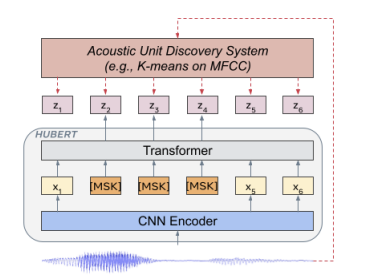
\includegraphics[width=70mm]{./img/HuBERT.png} 
\caption{{図 1}: HuBERTアプローチは、k-meansクラスタリングを1回または複数回繰り返すことで生成されたマスクされたフレーム(図中の \( y_2, y_3, y_4 \))の隠れクラスタ割り当てを予測する。}
\end{figure}

\section{実験}

\subsection{実験設定}

RVCを用いて変換された音声データを500、未変換の音声データを500、計1000のデータセットを作成した。その中から、ランダムサンプリングにより、訓練データとテストデータをそれぞれ400、100のデータセットを作成し、実験を行った。実験で使用したモデルは、従来手法であるCNNを用いたモデル、HuBERTを単体で用いたモデル、提案手法であるHuBERTとCNNを組み合わせたモデルの計3つである。これらのモデルに対して、入力された音声がRVCを用いて変換されたものか、そうでないかの2クラス分類を行うように学習した。


\subsection{結果}

CNNを用いたモデルによる推論結果は表1の通りである。
\vspace{5pt}
\begin{table}[htbp]
\centering
\caption{}
\begin{tabular}{cccc}
\toprule
Epoch & Training Loss & Validation Loss & Accuracy (\%) \\
\midrule
1 & 0.3538 & 0.2456 & 84.00 \\
2 & 0.1742 & 0.2422 & 88.00 \\
3 & 0.1368 & 0.2535 & 80.00 \\
4 & 0.1663 & 0.2592 & 80.00 \\
5 & 0.1886 & 0.2644 & 80.00 \\
6 & 0.1164 & 0.2791 & 80.00 \\
7 & 0.1543 & 0.2832 & 80.00 \\
8 & 0.2481 & 0.2811 & 80.00 \\
9 & 0.1784 & 0.2664 & 80.00 \\
10 & 0.1607 & 0.2556 & 80.00 \\
\bottomrule
\end{tabular}
\end{table}


また、HuBERTを単体で用いたモデルによる推論結果は表2のHuBERTとCNNを組み合わせてモデルによる推論結果は表3の通りである。
\vspace{10pt}
\begin{table}[htbp]
\centering
\caption{}
\begin{tabular}{cccc}
\toprule
Epoch & Training Loss & Validation Loss & Accuracy (\%) \\
\midrule
1  & 0.698800 & 0.695777 & 50.00 \\
2  & 0.694900 & 0.694842 & 50.00 \\
3  & 0.696400 & 0.693102 & 50.00 \\
4  & 0.690300 & 0.688122 & 50.00 \\
5  & 0.681000 & 0.665364 & 100.00 \\
6  & 0.657100 & 0.606551 & 100.00 \\
7  & 0.549300 & 0.524111 & 93.75 \\
8  & 0.489800 & 0.403892 & 93.75 \\
9  & 0.366900 & 0.325082 & 93.75 \\
10 & 0.262000 & 0.198047 & 100.00 \\
\bottomrule
\end{tabular}
\end{table}

\vspace{10pt}
\begin{table}[htbp]
\centering
\caption{}
\begin{tabular}{cccc}
\toprule
Epoch & Training Loss & Validation Loss & Accuracy (\%) \\
\midrule
1  & 0.684700 & 0.827347 & 37.50 \\
2  & 0.403900 & 0.329194 & 87.50 \\
3  & 0.245500 & 0.108115 & 100.00 \\
4  & 0.145500 & 0.075007 & 100.00 \\
5  & 0.036000 & 0.099326 & 93.75 \\
6  & 0.010700 & 0.340966 & 87.50 \\
7  & 0.005700 & 0.222607 & 93.75 \\
8  & 0.002300 & 0.067302 & 93.75 \\
9  & 0.001000 & 0.024201 & 100.00 \\
10 & 0.000500 & 0.035744 & 100.00 \\
\bottomrule
\end{tabular}
\end{table}

\subsection{実験の考察}

CNNを用いたモデルでは、少ないエッポクで精度が8割を超える結果となった。また、エポックを増やしたとしても安定した精度が出るため、ロバストな学習が可能である。しかし、精度が8割を超える程度なので、実用性を考えより高い精度を求める場合は、他の手法を用いる必要がある。次に、HuBERTを単体で用いたモデルでは、エポックを増やすにつれて精度とLossが上下し、安定した学習ができない。そこで、安定した精度で学習が可能なCNNと不安定だが高い精度を出すHuBERTを組み合わせたモデルを構築した。

結果としては表3から見えるように、HuBERTを単体で用いたモデルよりも、精度は少し落ちたもののどのエポックに対しても高い精度を出すことができ、Lossも安定して減少しておりロバストな学習が可能であることがわかった。

\section{課題と展望}
本研究では、オープンソースかつ少ないデータセットで高精度に学習元と同じ声のボイスチェンジャーを実現できるRVCを用いた。しかし、SO-VITS-SVC\cite{SO-VITS-SVC}.やYourTTS\cite{YourTTS}.など高精度なAIボイスチェンジャーが複数存在し、それらに対しても包括的かつ高精度に検出できるような研究が求められる。

\begin{thebibliography}{99}
  \bibitem{HuBERT} Wei-Ning Hsu, Benjamin Bolte, Yao-Hung Hubert Tsai, Kushal Lakhotia, Ruslan Salakhutdinov, Abdelrahman Mohamed, 
  "HuBERT: Self-Supervised Speech Representation Learning by Masked Prediction of Hidden Units", 
  arXiv:2106.07447, 2021.
  \bibitem{SO-VITS-SVC} \url{https://github.com/svc-develop-team/so-vits-svc}
  \bibitem{YourTTS}\url{https://github.com/Edresson/YourTTS}
\end{thebibliography}



\end{document}